\documentclass[12pt,a4paper]{book}
\usepackage[latin1]{inputenc}
\usepackage{amsmath}
\usepackage{amsfonts}
\usepackage{amssymb}
\usepackage{makeidx}
\usepackage{pdfpages}
\usepackage{fullpage}
\usepackage{listings}
\usepackage{color}

\definecolor{lightgray}{gray}{0.97}
%\lstset{frame=trBL}
\lstset{frame=single}
%\lstset{frameround=tttt}
\lstset{framesep=5pt}

%\lstset{rulecolor=\color{yellow}}
%\lstset{rulesepcolor=\color{green}}
%\lstset{fillcolor=\color{blue}}

\lstset{language=C++}
%\lstset{numbers=left, numberstyle=\tiny, stepnumber=2, numbersep=5pt}
\lstset{keywordstyle=\color{black}\bfseries\emph}
\lstset{backgroundcolor=\color{lightgray}}
%\lstset{emph={QwtPlot}}
%\lstset{emphstyle=\color{red}}

\author{Uwe Rathmann}
\title{Qwt Plot Framework}


\begin{document}

\maketitle
\pagestyle{headings}

\tableofcontents

\chapter{Introduction}

Introduction bla bla

\chapter{Plot Widget}

Plot widget bla bla.

\section{Composite Architecture}

Composite bla bla

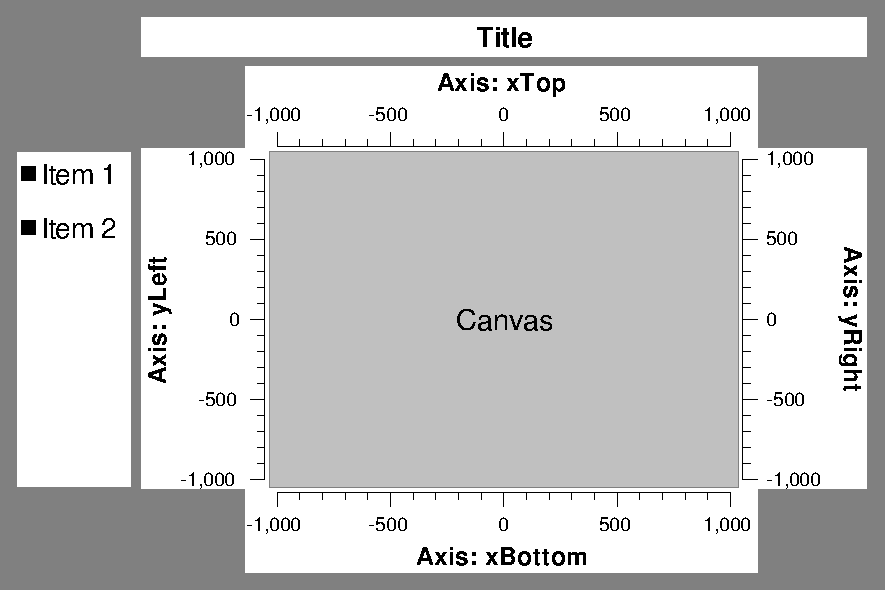
\includegraphics[scale=1.0]{plotlayout.pdf}

\section{Layout}

Bla Bla 

\begin{lstlisting}
#include <qwt_plot.h>

class MyPlot : public QwtPlot
{
public:
    ...
	
protected:
    virtual void doIt()
    {
        for ( int axis = 0; axis < QwtPlot::axisCnt; axis++ )
        ...
    }
};
\end{lstlisting}




Bla Bla

\section{Scale Widget}
\section{Legend}



\chapter{Scales, Axes and Transformations}

\section{Scale Divisions}

\section{Scale Maps}

\section{Scale Engine}

\section{Scale Renderer}

\chapter{Navigation and Selection}

\section{Picking}
\section{Zooming}
\section{Panning}

\chapter{Items on the Plot Canvas}

Decorations + items representing some sort of data.

\section{Overview}
\section{The Grid}
\section{Axes}

\section{Markers for Coordinates or Points}
\section{Curves displaying a series of 2D Points}

\subsection{Symbols}
\subsection{Styles}
\subsection{Curve Fitting}


\section{Curves displaying a series of 3D Points}
\section{Curves displaying a series of intervals}
\section{Histograms displaying ...}

\section{Spectrograms and other items displaying raster data}

\section{SVG Item}

\chapter{Exporting and Printing}

\chapter{Advanced Topics}

\section{Incremental Painting}

\section{Building Plot Grids}

\section{Controlling the Aspect Ratio}

\end{document}
